\documentclass[12pt,a4paper]{article}

% Margins.
\setlength{\oddsidemargin}{0in}
\setlength{\evensidemargin}{0in}
\setlength{\headheight}{12pt}
\setlength{\headsep}{0pt}
\setlength{\topmargin}{-60pt}
\setlength{\textwidth}{6.5in}
\setlength{\textheight}{10.75in}

\usepackage{amsmath}
\usepackage{float}
\usepackage{graphicx}
\usepackage[hyphens]{url}
\usepackage{hyperref}	% Clickable links to figures, references and urls.
\usepackage{datetime}
\usepackage{longtable}
\usepackage{array}

% Links direct to top of figures.
\usepackage[all]{hypcap}

% Drawing.
\usepackage{pgf}
\usepackage{tikz}

% Figures folder.
\graphicspath{{Figures/}}

% Listings for formatting code.
\usepackage{listings}
\usepackage{textcomp}

% Table cell alignment directives.
\newcolumntype{L}[1]{>{\raggedright\let\newline\\\arraybackslash\hspace{0pt}}m{#1}}
\newcolumntype{C}[1]{>{\centering\let\newline\\\arraybackslash\hspace{0pt}}m{#1}}
\newcolumntype{R}[1]{>{\raggedleft\let\newline\\\arraybackslash\hspace{0pt}}m{#1}}

% General options.
\lstset{breaklines=true, basicstyle=\footnotesize\ttfamily, tabsize=4, numbers=none, stepnumber=1, frame=single, showstringspaces=false, upquote=true}
% C++ specific high-lighting. Comments are 50/50 shades of green/black and strings coloured with 60/40 red/black mixture.
\lstset{language=[ISO]C++, commentstyle=\color{green!50!black}, keywordstyle=\color{blue}, stringstyle=\color{red!60!black}}

\newcommand\TotalMarks{60}
% Marks of each question
\def\Qone{5}
\def\Qtwo{15}
\def\Qthree{10}
\def\Qfour{20}
\def\Qfive{10}

%opening
\title{\LaTeX: Getting Started}
\author{}
\date{May 24, 2014\\[0.2cm] Last Modified: \today, \currenttime}
\begin{document}
\maketitle
\section{Introduction}
This is a tutorial that will get you started with \LaTeX~installation and a few basics. \LaTeX~is a typesetting program intended to produce high quality output especially designed for computing and engineering documentation needs. There is a learning curve but it isn't too steep and a lot of help is available online.
\section{Obtaining \LaTeX}
You can skip this section if you already have a working installation of \LaTeX. Before you can start using \LaTeX~you need to install two things:
\begin{enumerate}
\item The \LaTeX~compiler and packages suite: Output document type depends on compiler used. for example \verb|latex| produces \verb|.dvi| document and \verb|pdflatex| produces \verb|.pdf| document. Chances are you will have all these installed if using a popular distribution like \verb|Texlive| or \verb|MiKTeX|.
\item An editor: The most popular editor that works on both windows and linux is \verb|TeXstudio|. It was originally called \verb|TexMakerX|.
\end{enumerate}
\subsection{Installation on Windows}
\begin{enumerate}
\item Obtain the \verb|ProTeXt| bundle (a self--extracting \verb|exe| file) from \url{http://ctan.imsc.res.in/systems/windows/protext/} [fig. \ref{downloading-protext}]. The version available at the time of writing this tutorial is called \verb|ProTeXt-3.1.3-060313|.
\item Extract the \verb|ProTeXt| package [fig. \ref{protext-exe}] and run \verb|setup.exe| [fig. \ref{protext-setup}].
\item Select \verb|MiKTeX| [fig. \ref{miktex-install}] and choose `Complete' installation [fig. \ref{miktex-installation-type}] when prompted.
\item Install \verb|TexMakerX| or \verb|TeXstudio|, whichever came with your \verb|ProTeXt| package.
\item Start up \verb|TexMakerX|. Go to \verb|Options > Configure > Quick Build| and select\\ \verb|PdfLaTeX + View PDF| [fig. \ref{quickbuild-setup}]. Now you can compile and view your documents with the \verb|F1| key. This is not needed if using \verb|TeXstudio|.
\item A fresh installation of \verb|TeXstudio| may not detect correct path to \verb|MikTeX| installation. This can happen if pressing the \verb|F1| key or clicking on the double green arrow results in an error. To fix this, go to \verb|Options > Configure > Commands| and press all the buttons with yellow arrows to revert default paths.
\end{enumerate}
\subsection{Installation on Linux}
\begin{enumerate}
\item On terminal type \verb|yum install texlive| or \verb|apt-get install texlive| depending on your distribution package manager.
\item Install editor with \verb|yum install texmakerx| or \verb|yum install texstudio|. On debian based distributions use \verb|apt-get install texmakerx| or \verb|apt-get install texstudio| [fig. \ref{texstudio-paths}].
\end{enumerate}
\begin{figure}[H]
\centering
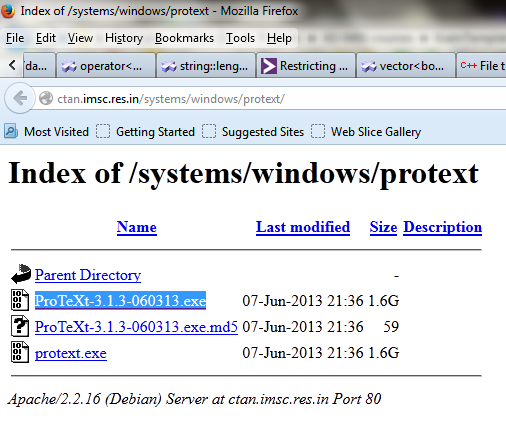
\includegraphics[scale=0.75]{Figures/DownloadProTeXt.png}
\caption{Downloading \texttt{ProTeXt}}
\label{downloading-protext}
\end{figure}
\begin{figure}[H]
\centering
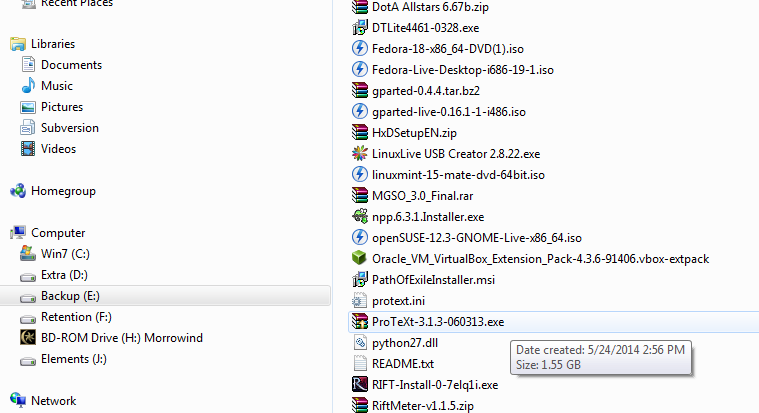
\includegraphics[scale=0.75]{ProTeXtexe.png}
\caption{\texttt{ProTeXt} executible}
\label{protext-exe}
\end{figure}
\begin{figure}[H]
\centering
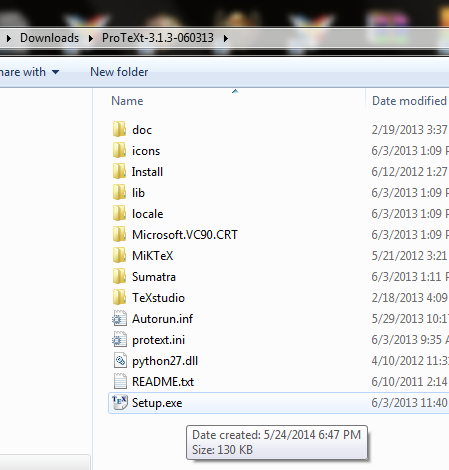
\includegraphics[scale=1.0]{ProTeXtSetup.png}
\caption{\texttt{ProTeXt} setup}
\label{protext-setup}
\end{figure}
\begin{figure}[H]
\centering
\includegraphics[scale=1.0]{MikTeXInstall.png}
\caption{\texttt{MikTeX} installation}
\label{miktex-install}
\end{figure}
\begin{figure}[H]
\centering
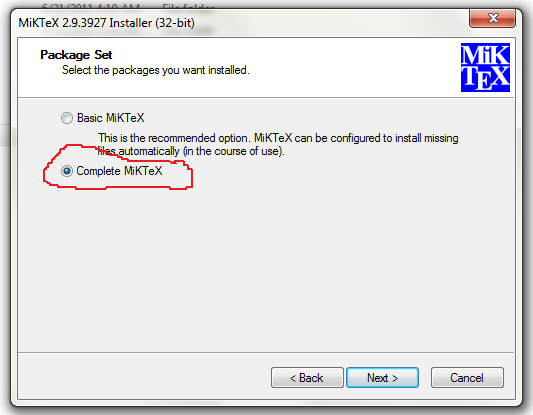
\includegraphics[scale=1.0]{MiKTeXComplete.png}
\caption{Selecting \texttt{MikTeX} installation type}
\label{miktex-installation-type}
\end{figure}
\begin{figure}[H]
\centering
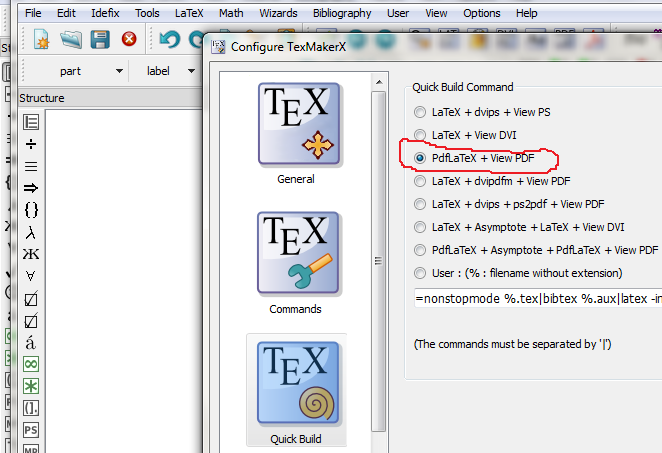
\includegraphics[scale=0.8]{QuickBuildSetup.png}
\caption{Quick build setup}
\label{quickbuild-setup}
\end{figure}
\begin{figure}[H]
\centering
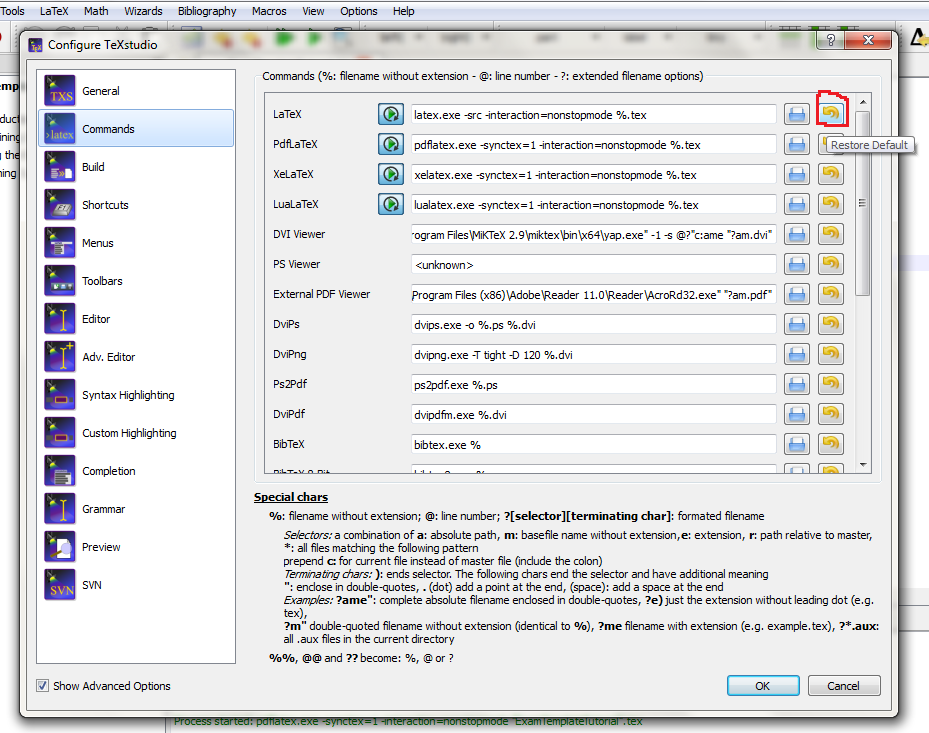
\includegraphics[scale=0.65]{TeXstudioPath.png}
\caption{Setting TeXstudio paths}
\label{texstudio-paths}
\end{figure}
\section{Basics}
\LaTeX~uses filetypes with \verb|.tex| extension as input. These files contain `code' to typeset the document. A \verb|.tex| file needs to be compiled into an output \verb|.pdf| file. The \verb|.tex| file can be opened in editor by double--clicking on it. Once opened, simply click the green arrow or press \verb|F1| to compile it [fig. \ref{build-and-view}]. Some temporary files will be created along with a \verb|.pdf| file. The editor also has a built--in viewer [fig. \ref{compiled}].

If the file is already open in Adobe Reader then compiling the \verb|.tex| file will generate an error saying that it cannot write on file.
\begin{figure}[h]
\centering
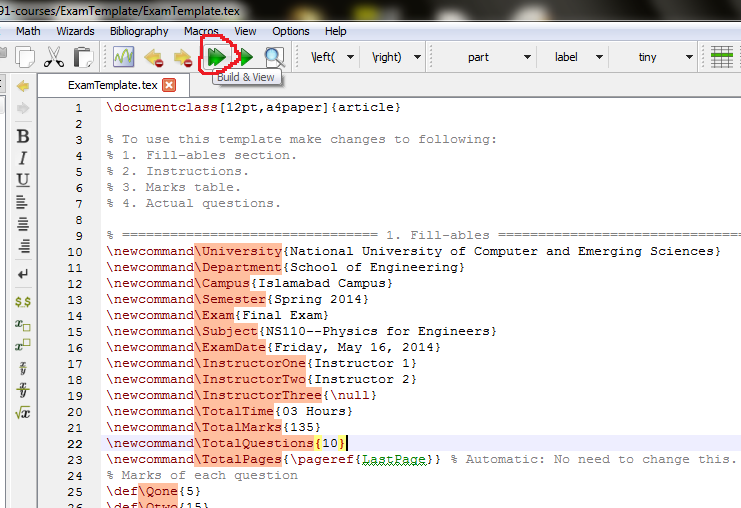
\includegraphics[scale=0.675]{BuildandView.png}
\caption{Building and viewing a document}
\label{build-and-view}
\end{figure}
\begin{figure}[h]
\centering
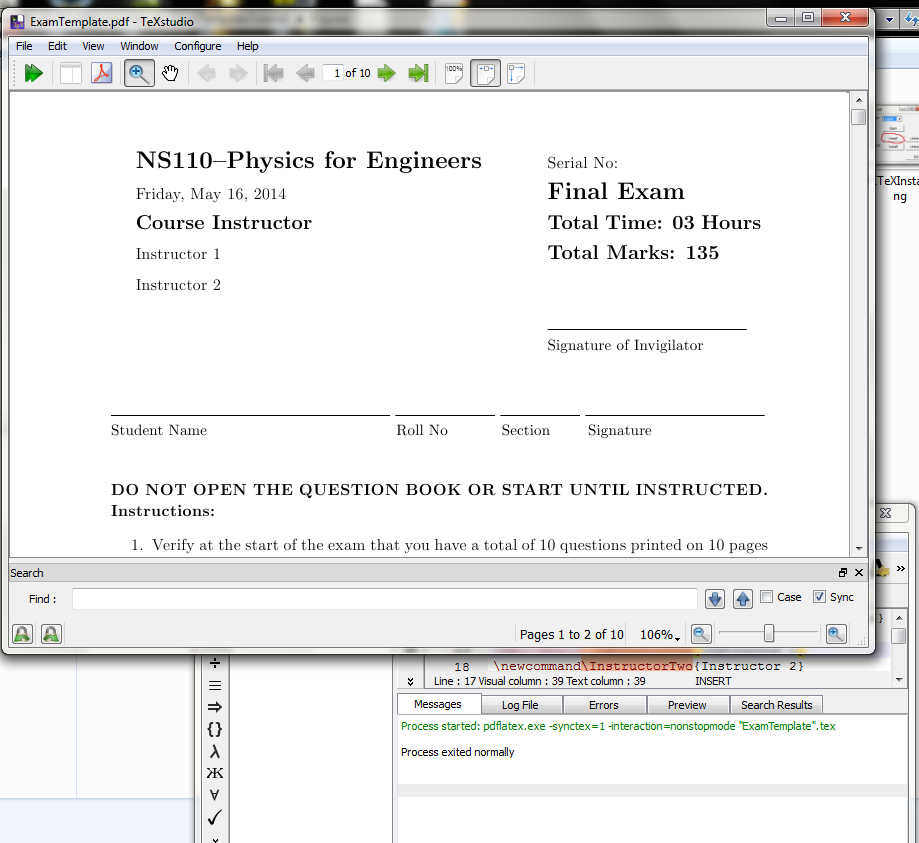
\includegraphics[scale=0.6]{Compiled.png}
\caption{Successful compilation}
\label{compiled}
\end{figure}
Here's an example of a simple exam question that is typeset as:
\begin{lstlisting}
\noindent\textbf{Question 1: Constructors/Destructors \hfill 10~marks}\\
Write the output of following program. Mention object name with constructor/destructor calls.
\end{lstlisting}
\begin{itemize}
\itemsep0em
\item A new paragraph begins with a little indentation or empty space. The \verb|\noindent| directive will remove this space.
\item Any text can be made bold with \verb|\textbf{bold text}|. This produces: \textbf{bold text}. The short cuts \verb|Ctrl+b| and \verb|Ctrl+i| can also be used to make the text bold or italic.
\item \verb|\hfill| will fill all horizontal space so that any following text is right-aligned. For example, \verb|I am left\hfill I am right| produces:\\I am left\hfill I am right
\item \verb|\\| starts a new line.
\item Equations are written inside a special math environment. The math environment is invoked with \verb|$|. The code \verb|$E=mc^2$| produces: $E=mc^2$.
\item Fractions can be written as \verb|\dfrac{numerator}{denominator}|.\\The code \verb|$\dfrac{1}{4}+\dfrac{1}{2}=\dfrac{3}{4}$| produces: $\dfrac{1}{4}+\dfrac{1}{2}=\dfrac{3}{4}$.
\item \LaTeX~treats multiple spaces as a single space. To insert multiple spaces use \verb|~|. The code \verb|four    spaces| produces: four    spaces. But the code \verb|four~~~~spaces| produces: four~~~~spaces.
\end{itemize}
\subsection{Working With Tables}
A table is created with the \verb|\begin{tabular}| directive. Additionally, number of columns in the table and text alignment must be specified with the \verb|\begin{tabular}| directive. A few examples are given below:
\lstset{language=TeX}
\begin{lstlisting}
% 1. A table with 3 columns and text center aligned. No separator between columns.
\begin{tabular}{c c c}

% 2. A table with 3 columns. Left-most column has left-aligned text. No separator.
\begin{tabular}{l c c}

% 3. A table with 4 columns and centre-aligned text. Columns are separated with a single vertical line.
\begin{tabular}{|c|c|c|c|}

% 4. A table with 4 columns and centre-aligned text. Columns are separated with a single vertical line. Width of left-most column is fixed at 1cm. Notice capital 'C'.
\begin{tabular}{|C{1.0cm}|c|c|c|}
\end{lstlisting}
Here's the code for a simple table. Width of left-most and right-most columns are fixed at 1.5 cm and 3 cm respectively. Width of middle two columns is automatic and they are centre-aligned. Left-most column is left-aligned and right-most column is right-aligned. An \verb|&| ends a column. The last column is ended with newline directive \verb|\\|.\newpage
\begin{lstlisting}
\begin{tabular}{|L{1.5cm}|c|c|R{3cm}|}
\hline
	R1C1 & R1C2 & R1C3 & R1C4 \\ % Row 1
\hline
	R2C1 & R2C2 & R2C3 & R2C4 \\ % Row 2
\hline\hline
\end{tabular}
\end{lstlisting}
This produces:
\begin{tabular}{|L{1.5cm}|c|c|R{3cm}|}
\hline
	R1C1 & R1C2 & R1C3 & R1C4 \\
\hline
	R2C1 & R2C2 & R2C3 & R2C4 \\
\hline\hline
\end{tabular}
The \verb|\hline| draws a horizontal line between two rows. There are two lines after last row. If we want to remove third column from the table the modified code would be:
\begin{lstlisting}
\begin{tabular}{|L{1.5cm}|c|R{3cm}|}
\hline
	R1C1 & R1C2 & R1C4 \\ % Row 1
\hline
	R2C1 & R2C2 & R2C4 \\ % Row 2
\hline\hline
\end{tabular}
\end{lstlisting}
And the code produces:
\begin{tabular}{|L{1.5cm}|c|R{3cm}|}
\hline
	R1C1 & R1C2 & R1C4 \\
\hline
	R2C1 & R2C2 & R2C4 \\
\hline\hline
\end{tabular}\\
\underline{The number of \&'s in a single row must exactly be equal to one less than total columns.}
\section{Learning \LaTeX}
There are several \LaTeX~tutorials available online. Following two tutorials are an excellent resource.
\begin{enumerate}
%\item A good place to start learning basics of \LaTeX~is: \url{http://en.wikibooks.org/wiki/LaTeX/Basics}
\item \url{https://www.tug.org/twg/mactex/tutorials/ltxprimer-1.0.pdf}.
\item \url{http://tobi.oetiker.ch/lshort/lshort.pdf}
\end{enumerate}
%\nocite{*}
%\bibliographystyle{plain}
%\bibliography{PhysicsRef}
\end{document}
